\documentclass{article}
\usepackage{fullpage,graphicx}
\usepackage{amsmath,amsfonts,amsthm,amssymb,multirow, url}
\usepackage{tikz}
\usepackage{wrapfig}
\usepackage{algorithmic}
\usepackage[ruled,vlined,commentsnumbered,titlenotnumbered]{algorithm2e}
\newcommand{\expecting}[1]{\noindent{[\textbf{We are expecting:} \em #1\em]}}
\newcommand{\pts}[1]{\textbf{(#1 pt.)}}


\begin{document}
\noindent
CS 161 \hfill \textbf{Problem Set 1} \newline 
{Winter 2019} \hfill \textbf{Due:} Friday, January 18, 2019 at 3pm on Gradescope.

\noindent
\rule{\linewidth}{0.4pt}

\noindent
\textbf{Style guide and expectations:} Please see the ``Homework" part of the ``Resources" section on the webpage for guidance on what we are looking for in homework solutions.  We will grade according to these standards.
\newline\newline
Make sure to look at the ``\textbf{We are expecting}'' blocks below each problem to see what we will be grading for in each problem!

\section*{Exercises}
Please do the exercises on your own.

\noindent
\rule{\linewidth}{0.4pt}
\begin{enumerate}

%%%%%%%%%%

\item[0.] \pts{1} Have you thoroughly read the course policies on the webpage?

\expecting{The answer ``yes."}

%%%%%%%%%%%

\item \pts{1} See the IPython notebook \texttt{HW1.ipynb} for Exercise 1.  Modify the code to generate a plot that convinces you that $T(x) = O(g(x))$. \textbf{Note:} There are instructions for installing Jupyter notebooks in the pre-lecture exercise for Lecture 2.

\expecting{Your choice of $c$, $n_0$, the plot that you created after modifying the code in Exercise 1, and a short explanation of why this plot should convince a viewer that $T(x) = O(g(x))$.}

%%%%%%%%%%%

\item \pts{3} See the IPython notebook \texttt{HW1.ipynb} for Exercise 2, parts A, B and C.
\begin{itemize}
	\item[(A)] What is the asymptotic runtime of the function \texttt{numOnes( lst )} given in the Python notebook?  Give the smallest answer that is correct.  (For example, it is true that the runtime is $O(2^n)$, but you can do better).

	\expecting{Your answer in the form ``The running time of \texttt{numOnes( lst )} on a list of size $n$ is $O(\_\_\_)$.", and a short explanation of why this is the case. }

	\item[(B)] Modify the code in \texttt{HW1.ipynb} to generate a picture that backs up your claim from Part (A).

	\expecting{Your choice of $c$, $n_0$, and $g(n)$; the plot that you created after modifying the code in Exercise 2; and a short explanation of why this plot should convince a viewer that the runtime of \texttt{numOnes} is what you claimed it was.}

	\item[(C)] How much time do you think it would take to run \texttt{numOnes} on an input of size $n = 10^{15}$?

\expecting{Your answer (in whichever unit of time makes the most sense) with a short explanation that references the runtime data you generated in part (B).  You don't need to do any fancy statistics, just a reasonable back-of-the-envelope calculation.}
\end{itemize} 

%%%%%%%%%%%

\item \pts{4} Using the definition of big-Oh, formally prove the following statements.
\begin{enumerate}
	\item $3\sqrt{n} + 2 = O( \sqrt{n} )$  (Note that you gave a ``proof-by-picture" of this in Exercise 1).
	\item $n^2 = \Omega(n)$.
	\item $2^{2^{2^{100}}} = \Theta(1)$. 
	\item $4^n$ is \textbf{not} $O(2^n)$.
\end{enumerate}
\expecting{A proof for each part, using the definition of $O(), \Omega()$, and $\Theta()$.}

\end{enumerate}

\noindent
\rule{\linewidth}{0.4pt}
\newpage
\section*{Problems}
You may talk with your fellow CS161-ers about the problems.  However:
\begin{itemize}
	\item Try the problems on your own \em before \em collaborating.
	\item Write up your answers yourself, in your own words.   You should never share your typed-up solutions with your collaborators.
	\item If you collaborated, list the names of the students you collaborated with at the beginning of each problem.
\end{itemize}

\noindent
\rule{\linewidth}{0.4pt}

\begin{enumerate}
\item \textbf{[True or false?]} \pts{4}
In the following, suppose that $f:\mathbb{N} \to \mathbb{N}$ and $g:\mathbb{N} \to \mathbb{N}$ are strictly increasing functions.  (Recall that $\mathbb{N}$ denotes the natural numbers $\{0,1,2,\ldots\}$).


True or false?
\begin{enumerate}
\item \pts{2} If $f(n) = O(g(n))$, then $\log(f(n)) = O( \log(g(n)) )$.  (If it helps, you may assume that $f$ and $g$ are strictly positive).
\item \pts{2} If $f(n) = O(g(n))$, then $2^{f(n)} = O\left( 2^{g(n)} \right)$.
\end{enumerate}
\expecting{For each part, either a proof or a counter-example (along with a proof that your counter-example is a counter-example), using the definition of $O(\cdot)$.}

%%%%%%%%%%%%%%%

\item \textbf{[Alternative MergeSorts]} \pts{6} 

In class, we saw how \textsc{MergeSort} works by recursively breaking up a list into two smaller lists.  Consider the following version, which recursively breaks a list up into three smaller lists:

\begin{verbatim}
# Assume that A is a list of distinct integers and len(A) is a power of 3.
# This function returns a sorted version of A.
def MergeSort3(A):
     n = len(A)
     if n <= 3:
         return InsertionSort(A)     
            # It takes time O(1) to InsertionSort a list of length <= 3. 
     L = MergeSort3(A[0:n/3])
     M = MergeSort3(A[n/3:2n/3])
     R = MergeSort3(A[2n/3:n])
     return Merge3(L,M,R)  
         # Merge3 merges three sorted lists of size n/3 into a sorted list of size n.
\end{verbatim}

\begin{enumerate}
\item \pts{2} Write pseudocode for \texttt{Merge3} that runs in time $O(n)$.  Your function should take as input three sorted lists \texttt{L}, \texttt{M}, and \texttt{R} of length $n/3$ (where $n$ is a power of $3$) and return a sorted list of length $n$ which contains all the entries of \texttt{L} and \texttt{M} and \texttt{R}.

\expecting{Pseudocode \textbf{AND} an English description of what it does, as well as an informal explanation of why the running time is $O(n)$. You may assume that $n$ is a power of $3$ and that all of the elements across \texttt{L,M,R} are distinct.}
\item \pts{2} Show that, with your version of \texttt{Merge3} from part (a), \texttt{MergeSort3} runs in time $O(n \log(n))$ when run on a list of length $n$.

\expecting{An informal but convincing argument.  Do not use the Master Theorem, instead argue this ``from scratch'' like we did in Lecture 2.}

\vfill\hfill (More parts on next page...)
\newpage
\item \pts{2}
Your friend has gotten pretty excited by this, and thinks they have a sorting algorithm that runs in time $O(n \log\log(n))$, even faster than \textsc{MergeSort}.  Here is their reasoning:

\begin{enumerate}
\item Instead of \texttt{MergeSort3} as above, consider a version \texttt{MergeSort\_k} which breaks up the list $A$ recursively into $k$ parts, and uses a routine \texttt{Merge\_k} similar to the \texttt{Merge3} you wrote in part (a).
\item The routine \texttt{Merge\_k} takes $k$ sorted lists of size $n/k$, and returns a sorted list of size $n$.  Your approach in part (a) still applies: we've already seen that \texttt{Merge\_k} runs in time $O(n)$ for $k=2$ and $k=3$, and it's not hard to see that the natural generalization also runs in time $O(n)$ for $k=4,5,6, \ldots$.  
\item Now instantiate this algorithm \texttt{MergeSort\_k} for $k = \sqrt{n}$.  That is, at each step we divide a list of size $n$ into $\sqrt{n}$ pieces of size $\sqrt{n}$, and recurse on those.  (For simplicity, assume that $n$ is of the form $n= 2^{2^t}$ for some $t$ so that $\sqrt{n}$ and $\sqrt{ \sqrt{n} }$ and so on is always an integer until $n=2$.)
\item Now we have a recursive algorithm with the following properties:
\begin{itemize}
	\item A problem of size $n$ gets broken up into $\sqrt{n}$ problems of size $\sqrt{n}$. 
	\item The work to run \texttt{Merge\_}$\sqrt{n}$ for a subproblem of size $n$ is $O(n)$ by part (ii).
\end{itemize}
The running time is $O(n \log\log(n))$.  
To see this, first notice that there are $O(\log\log(n))$ levels in the recursion tree, since that's how many times you need to take the square root of $n$ to get down to problems of size $O(1)$.  At the $0$'th level of the recursion tree, there is one problem of size $n$.  At level $1$, there are $\sqrt{n}$ problems of size $\sqrt{n}$.  At level $2$, there are $\sqrt{n}\cdot n^{1/4} = n^{3/4}$ problems of size $n^{1/4}$.  In general, at the $j$'th level there are $n^{1 -1/2^j}$ problems of size $n^{1/2^j}$.  Thus, the amount of work at level $j$ is $O(n^{1-1/2^j} \cdot n^{1/2^j} ) = O(n)$.  Thus, since there is $O(n)$ work per layer for each of $O(\log\log(n))$ layers, the total amount of work is $O(n \log\log(n) )$.
\end{enumerate}

This is pretty neat!  Unfortunately, it's not correct.  What is the problem with your friend's argument?  (Don't go looking for little bugs---there is a big conceptual error.  The assumption that $n$ is of the form $2^{2^t}$ is fine.)

\expecting{An identification of which step(s) of the argument (i)-(iv) are problematic, and a clear explanation about what is wrong.}
\end{enumerate}

%%%%%%%%%%%%%%%

\vfill
\hfill
(More questions on next page...)

\newpage
\item \textbf{[Nuts!]} \pts{8} 

\begin{minipage}{.55\textwidth}
Socrates the Scientific Squirrel is conducting some experiments.
Socrates lives in a very tall tree with $n$ branches, and she wants to find out what is the lowest branch $i$ so that an acorn will break open when dropped from branch $i$.  (If an acorn breaks open when dropped from branch $i$, then an acorn will also break open when dropped from branch $j$ for any $j \geq i$.)

\vspace{.3cm}
The catch is that, once an acorn is broken open, Socrates will eat it immediately and it can't be dropped again.

\begin{enumerate}
\item[(a)] \pts{2} Suppose that Socrates has $\lceil\log(n)\rceil + 1$ acorns.  Give a procedure so that she can identify the correct branch using $O(\log(n))$ drops.

\expecting{Very clear pseudocode or a short English description of your algorithm.  You do not need to justify the number of drops.  If it helps you may assume that $n$ is a power of $2$.}
\end{enumerate}
\end{minipage}
\hspace{.5cm}
\begin{minipage}{.4\textwidth}
\hfill
\begin{tikzpicture}
\node{
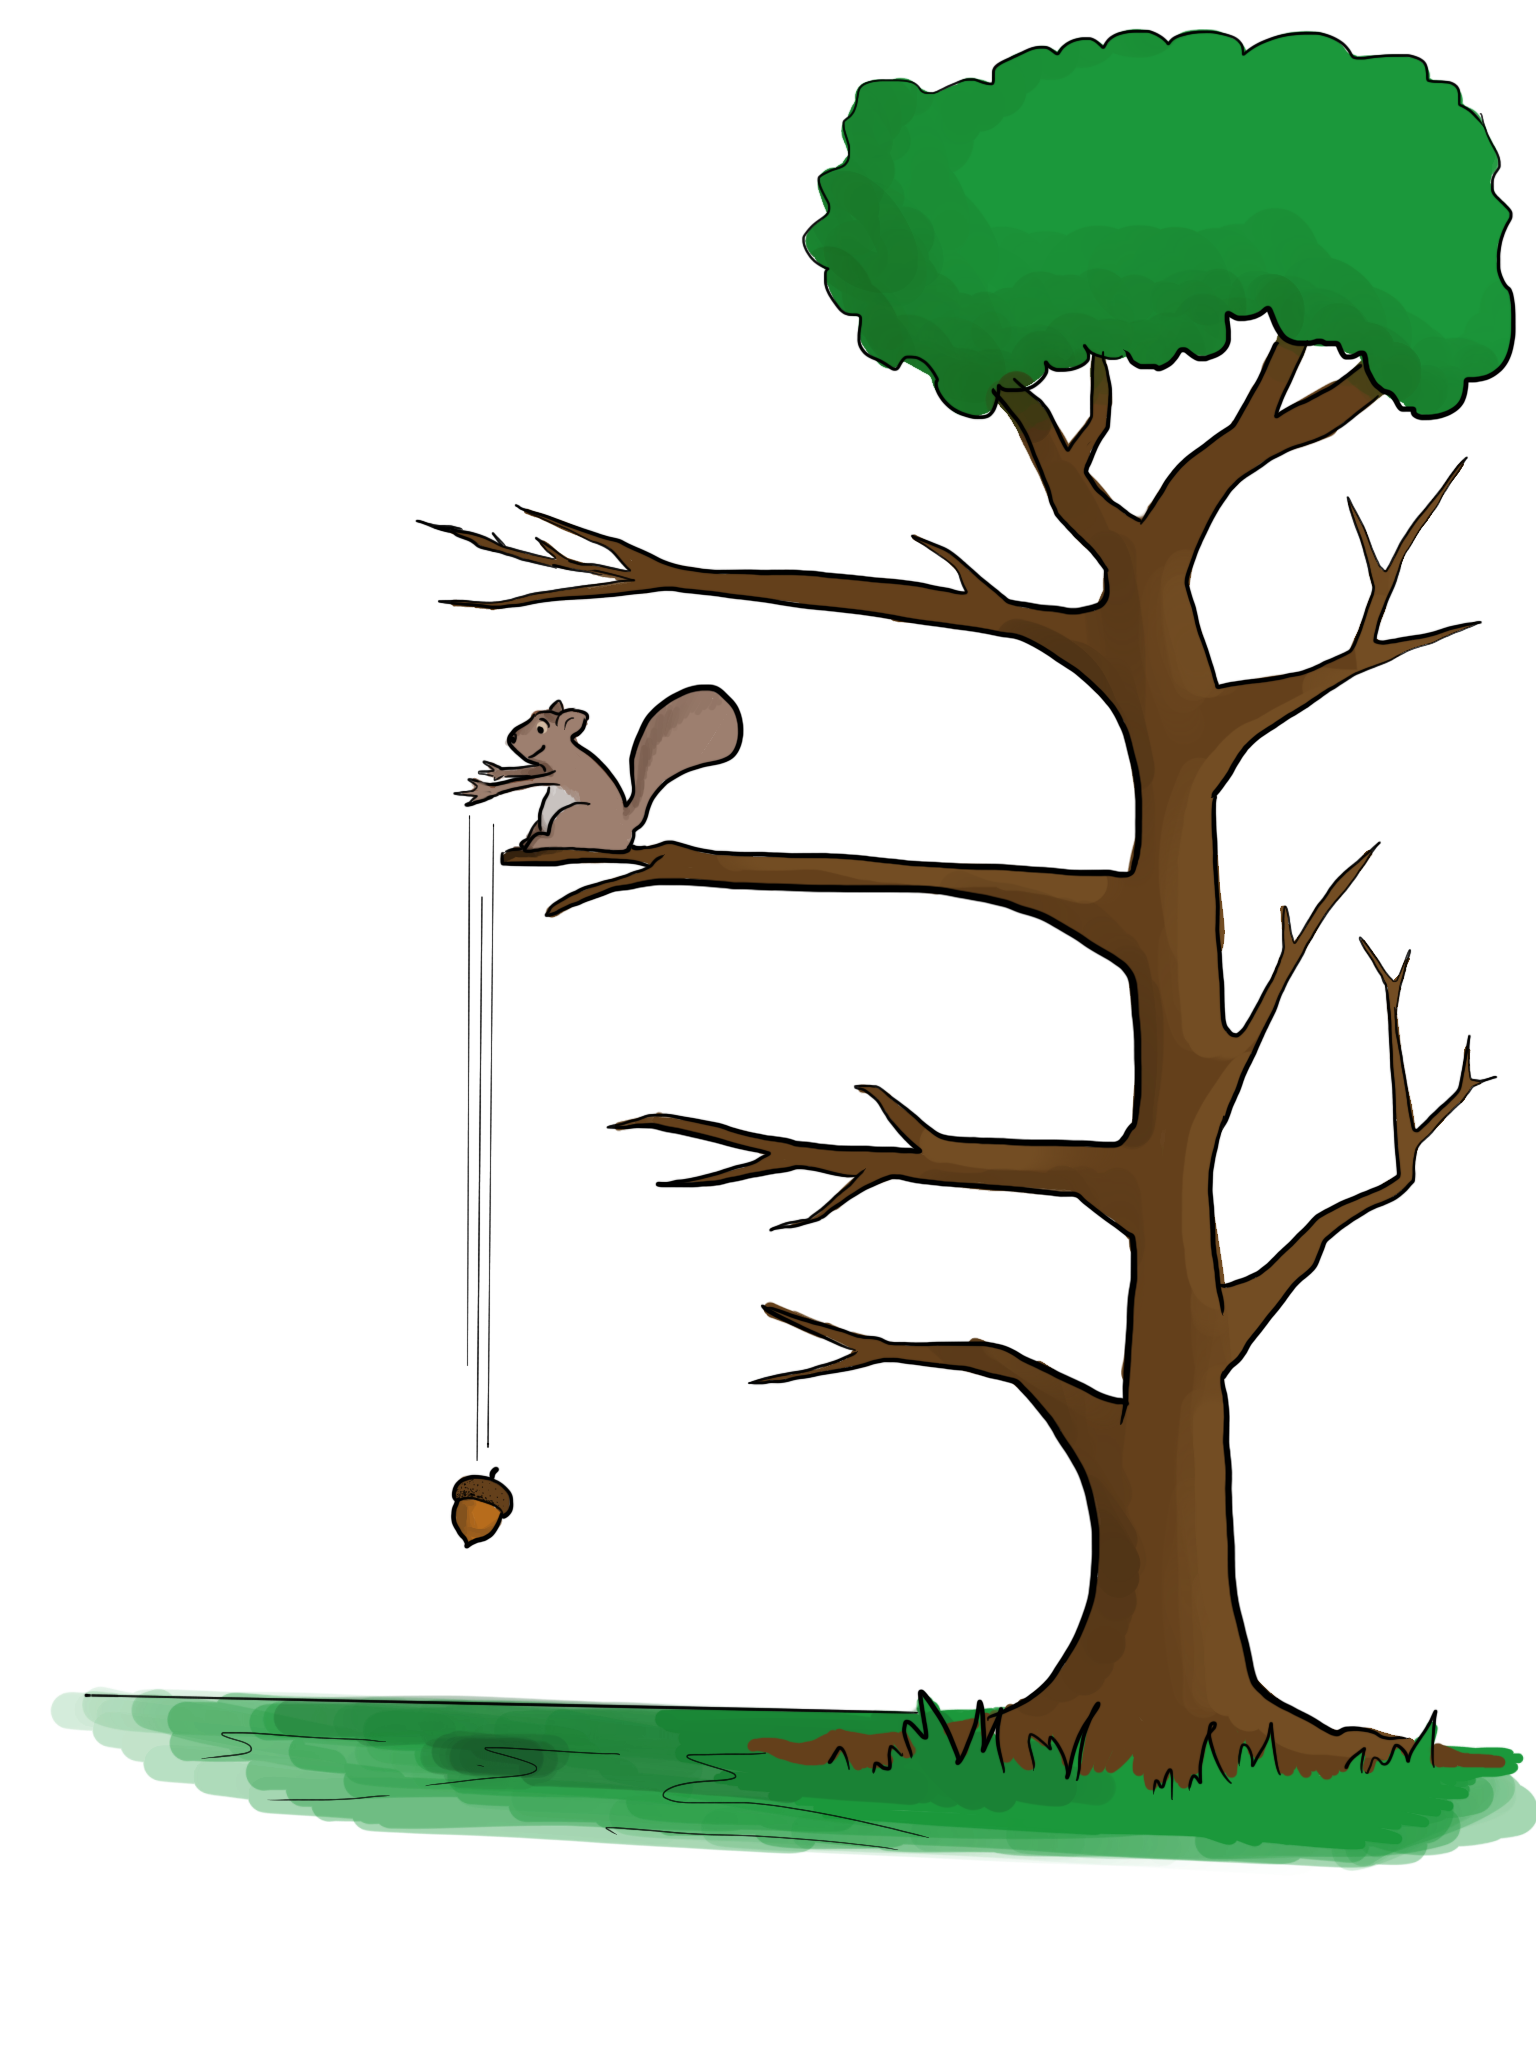
\includegraphics[width=6cm]{squirrel}};
\node(bn) at (-2.5,1.8) {Branch $n-1$};
\node(b0) at (-2.2,-1.25) {Branch $0$};
\node(b1) at (-2.2,-.55) {Branch $1$};
\draw(b0) -- (-.3, -1.25);
\draw(b1) -- (-.7, -.55);
\end{tikzpicture}
\end{minipage}

\begin{enumerate}
\item[(b)] \pts{1} Suppose that Socrates has only one acorn.  Give a procedure so that she can identify the correct branch using $O(n)$ drops, and explain why your $O(\log(n))$-drop solution from part (a) won't work.

\expecting{Very clear pseudocode or a short English description of your algorithm, and one sentence about why your algorithm from part (a) does not apply.  You do not need to justify the number of drops.}

\item[(c)] \pts{2} Suppose that Socrates has two acorns.  Give a procedure so that she can identify the correct branch using $O(\sqrt{n})$ drops.

\expecting{Pseudocode \textbf{AND}  a short English description of your algorithm, and a justification of the number of drops.  If it helps you may assume that $n$ is a perfect square.}

\item[(d)] \pts{2} Suppose that Socrates has $k = O(1)$ acorns.  Give a procedure so that she can identify the correct branch using $O(n^{1/k})$ drops.

\expecting{Pseudocode \textbf{AND} a short English description of your algorithm, and a justification of the number of drops.  If it helps you many assume that $n$ is of the form $n = m^k$ for some integer $m$.}

\item[(e)] \pts{1} What happens to your algorithm in part (d) when $k = \lceil \log(n) \rceil + 1$?  
Is it $O(\log(n))$, like in part (a)? Is it $O(n^{1/k})$ when $k=\lceil \log(n) \rceil + 1$, like in part (d)?  

\expecting{A sentence of the form ``the number of drops of my algorithm in part (d) when $k=\lceil \log(n) \rceil + 1$ is $O(\_\_\_\_)$'', along with justification.  Also, two yes/no answers to the two yes/no questions (you should justify your answers but do not need to include a formal proof). }

\item[(f)] \pts{NOT REQUIRED.  1 BONUS} Is $\Theta(n^{1/k})$ drops is the best that Socrates can do with $k$ acorns, for $k = O(1)$?  Either give a proof that she can't do better, or give an algorithm with asymptotically fewer drops.

\expecting{Nothing.  This part is not required.}

\end{enumerate}

\end{enumerate}

\rule{\linewidth}{0.4pt}
\section*{Feedback}
This part is not worth any points, but it is quick, painless, and anonymous, and we'd really appreciate it if you'd help us out by giving us feedback! 
\begin{enumerate}
\item \pts{0} Please fill out the following poll, which asks about your expectations for the course: 
\begin{center} \url{https://goo.gl/forms/RKAgpsDPu2IT9RWE3} \end{center}
\end{enumerate}

\end{document}
